\documentclass[11pt]{beamer}
\mode<presentation>
%\documentclass[handout,compress]{beamer}
\usepackage{beamerthemedefault}
\usepackage{graphicx}
\usepackage{hyperref}
\usepackage{subfigure}
\usepackage{color}
\usepackage{multicol}
\usepackage{bm} 
\usepackage{tikz}
\usepackage{listliketab}

\usetheme{CambridgeUS}
\makeatletter
\makeatother
\usetikzlibrary{shapes,backgrounds}
\tikzstyle{cblue}=[circle, draw, thin,fill=cyan!20, scale=0.8]
\tikzstyle{qgre}=[rectangle, draw, thin,fill=green!20, scale=0.8]
\tikzstyle{rpath}=[ultra thick, red, opacity=0.4]
\tikzstyle{legend_isps}=[rectangle, rounded corners, thin,
fill=gray!20, text=blue, draw]
\usetikzlibrary{decorations.pathreplacing}
\tikzset{text/.default=}
%\tikzset{text/.align=0}
\tikzstyle{every picture}+=[remember picture]
\tikzstyle{na} = [baseline=-.5ex]
\setbeamertemplate{itemize item}{\color{black}$\bullet$}
\setbeamertemplate{itemize subitem}{\color{black}$\bullet$}

\usetikzlibrary{shapes}
\usetikzlibrary{positioning}
\usetikzlibrary{automata}
\usepackage{amsmath,amssymb,amsfonts,amsthm}
\setbeamercovered{invisible} %% <--- I ADDED THIS
\newcommand{\red}{\textcolor{red}}
\newcommand{\blue}{\textcolor{blue}}
\newcommand{\purple}{\textcolor{purple}}
\newcommand{\brown}{\textcolor{brown}}
\newcommand{\cyan}{\textcolor{cyan}}
\newcommand{\real}{\ensuremath{\mathbb{R}}}
\newcommand{\y}{\ensuremath{\mathbf{y}}}
\newcommand{\black}{\color{black}}
\newcommand{\btheta}{\boldsymbol{\theta}}
\newcommand{\green}{\color{green}}
\newcommand{\word}[1]{\green{\textit{#1}\ }\black}
\newcommand{\lb}{\linebreak}
\newtheorem{com}{Comment}
\newtheorem{lem} {Lemma}
\newtheorem{prop}{Proposition}
\newtheorem{thm}{Theorem}
\newtheorem{defn}{Definition}
\newtheorem{cor}{Corollary}
\newtheorem{obs}{Observation}
\setcounter{tocdepth}{1}

\definecolor{UBCblue}{rgb}{0.04706, 0.13725, 0.26667}
\definecolor{UBCgray}{rgb}{0.3686, 0.5255, 0.6235}
\colorlet{verylightgray}{gray!10}
\setbeamercolor{palette primary}{bg=UBCblue,fg=white}
\setbeamercolor{palette secondary}{bg=darkgray,fg=white}
\setbeamercolor{palette tertiary}{bg=UBCblue,fg=white}
\setbeamercolor{palette quaternary}{bg=UBCblue,fg=white}
\setbeamercolor{structure}{fg=UBCblue} % itemize, enumerate, etc
\setbeamercolor{section in toc}{fg=UBCblue} % TOC sections
\setbeamercolor{subsection in head/foot}{bg=darkgray,fg=white}
\setbeamercolor{frametitle}{fg=UBCblue}
\setbeamercolor{title}{fg=UBCblue, bg=verylightgray}

\title[Class 9]{Introduction to Social Data Analytics \\
	\bigskip Week 5: Class 9}
\author[Kaushik]{Arushi Kaushik}
\institute[UCSD]{arkaushi@ucsd.edu}
\date[Data Wrangling in Stata- I]{}

% update title block above

\begin{document}

\frame{\titlepage}

%\begin{frame}
%    \frametitle{Housekeeping}
%    \begin{itemize} \itemsep1em
%    \item Problem Set 2 due this morning
%    \item Quiz 3 due this Wednesday (9AM)
%    \item Stata plotting today, regression Wednesday
%    \item Review for midterm next week on Monday
%    \end{itemize}
%\end{frame}

\begin{frame}
\frametitle{Today: Data Wrangling in Stata}
By the end of today's lecture, you should be able to: \medskip
\begin{itemize} \itemsep1em
	\item Demonstrate appending and merging data
	\item Generate identifiers to differentiate between observations within a group 
	\item Explain the difference between 1:1 and m:1 merges
	%\item Collapse a dataset to a coarser unit of analysis
\end{itemize} \bigskip
Open class9.do if you haven't already. 
\end{frame}

\begin{frame}
\frametitle{Appending vs Merging}
We \alert{append} data to add observations, or rows. \\ \bigskip
We \alert{merge} data to add variables, or columns. 
\end{frame}

\begin{frame}
\frametitle{Append to combine observations from tables with common variables}
\begin{center}
	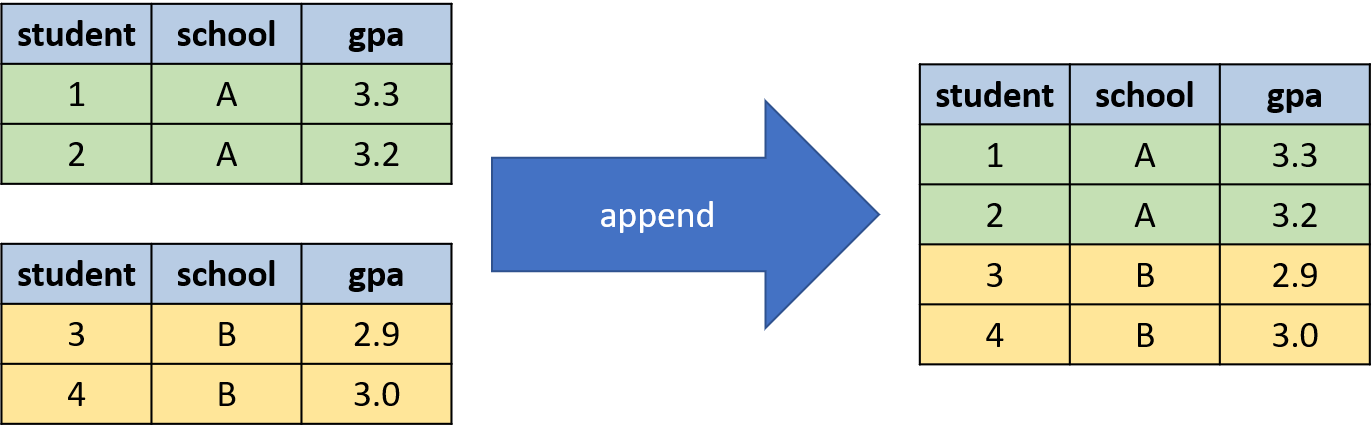
\includegraphics[width=\textwidth]{images/append.png}
\end{center} %\pause \bigskip
%From the pre class exercise: \texttt{append using person2016}
\end{frame}


\begin{frame}
\frametitle{Append to combine observations from tables}
\begin{center}
	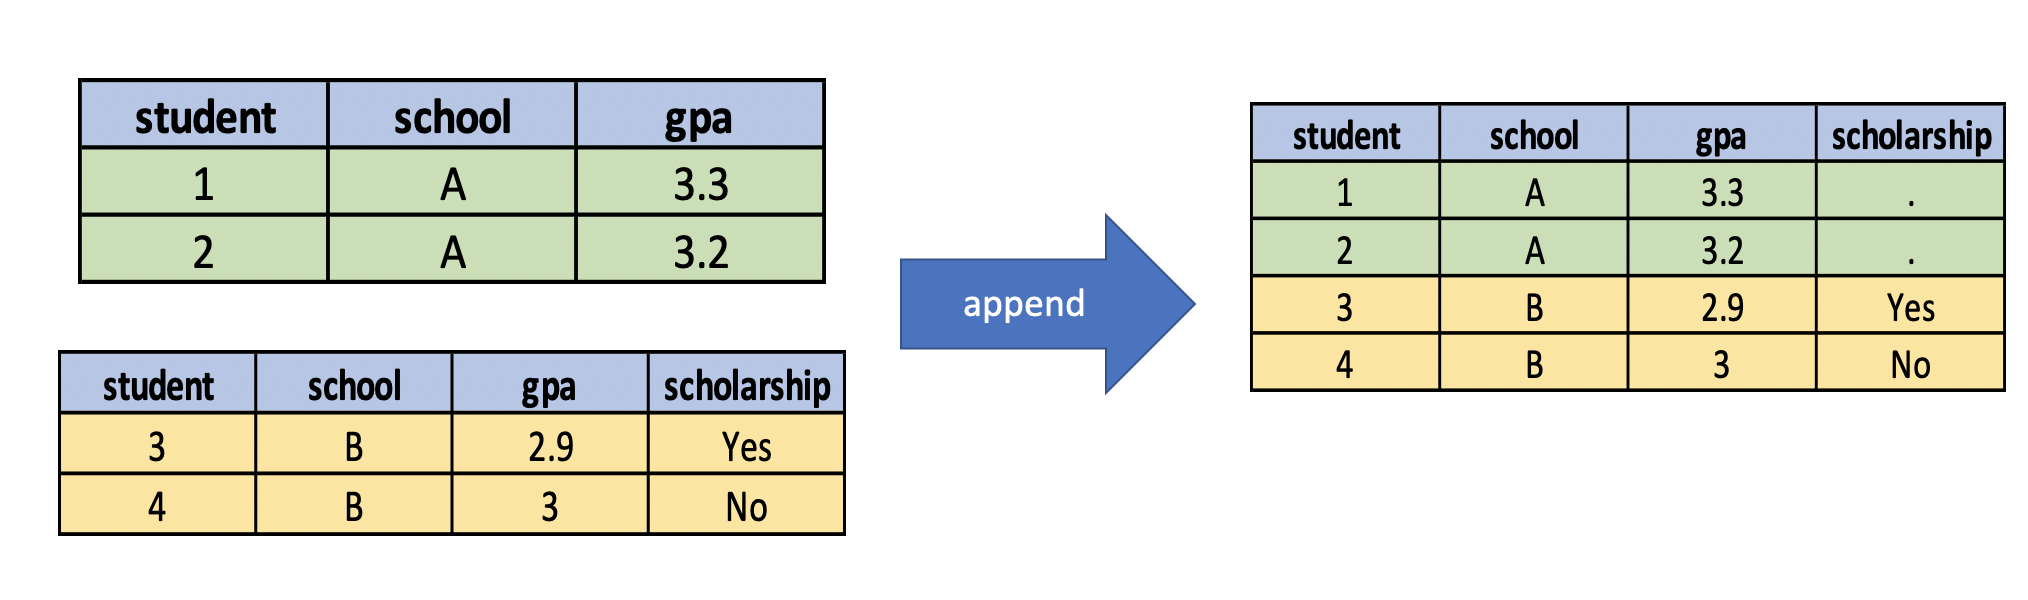
\includegraphics[width=\textwidth]{images/append2.png}
\end{center} 
If there are variables that exist \textbf{only in one} of the datasets, the datasets can still be appended
%\pause \bigskip
%From the pre class exercise: \texttt{append using person2016}
\end{frame}


\begin{frame}
\frametitle{Class exercise: \textit{append}}
\begin{itemize}
\item Open \texttt{class9.do} 
\item Open \texttt{person2015} dataset
\item \texttt{append using person2016}
\item \texttt{append using person2017}
\item save as \texttt{combined\_worker.dta} file
\end{itemize}
\end{frame}



\begin{frame}
\frametitle{Merge 1:1 when both tables have same unit of analysis}
\begin{center}
	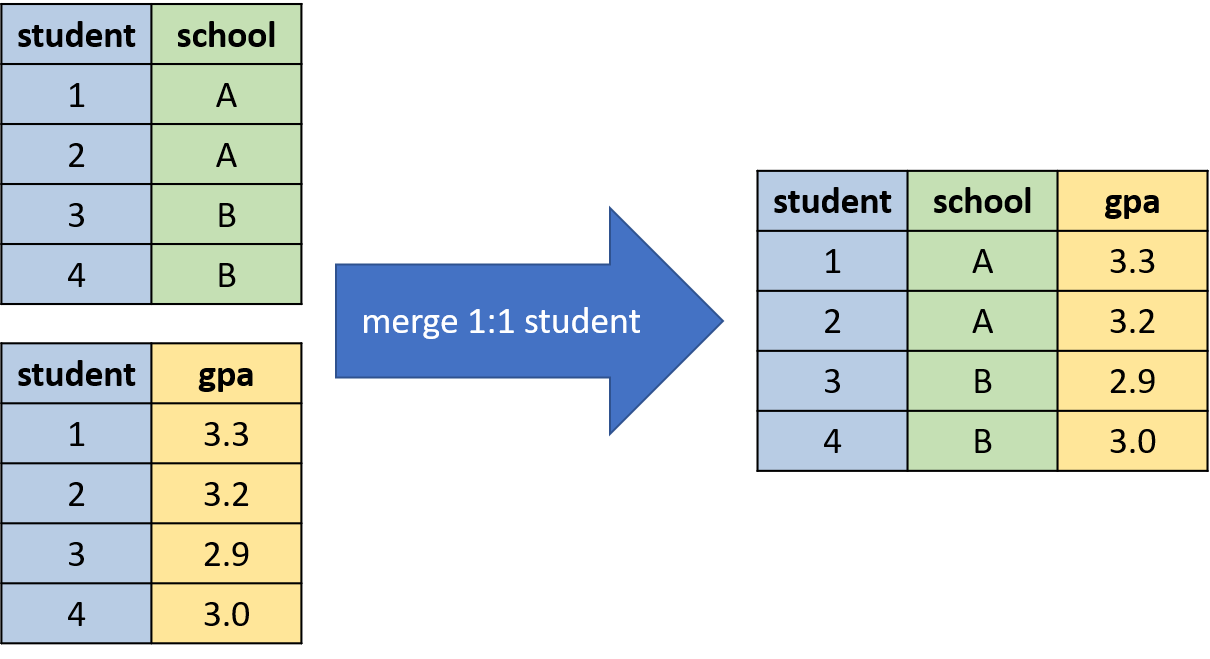
\includegraphics[width=0.9\textwidth]{images/merge_one.png}
\end{center} 
\end{frame}


\begin{frame}
\frametitle{Class exercise: \textit{merge 1:1}}
\begin{itemize}
\item Open \texttt{class9.do} 
\item Open \texttt{demographics.dta} dataset \\
\bigskip
We'll merge the \texttt{combined\_worker.dta} with the demographics data\\
\bigskip
\item Verify that \textbf{year-id} is the unique identifier in both datasets
\item \texttt{sort year id}
\item \texttt{merge 1:1 year id using "combined\_worker.dta", gen(\_merge)}
\item save as \texttt{class9.dta} file
\end{itemize}
\end{frame}


\begin{frame}
\frametitle{Merge m:1 when one table has a coarser unit of analysis}
What is the unit of analysis of each table?
\begin{center}
	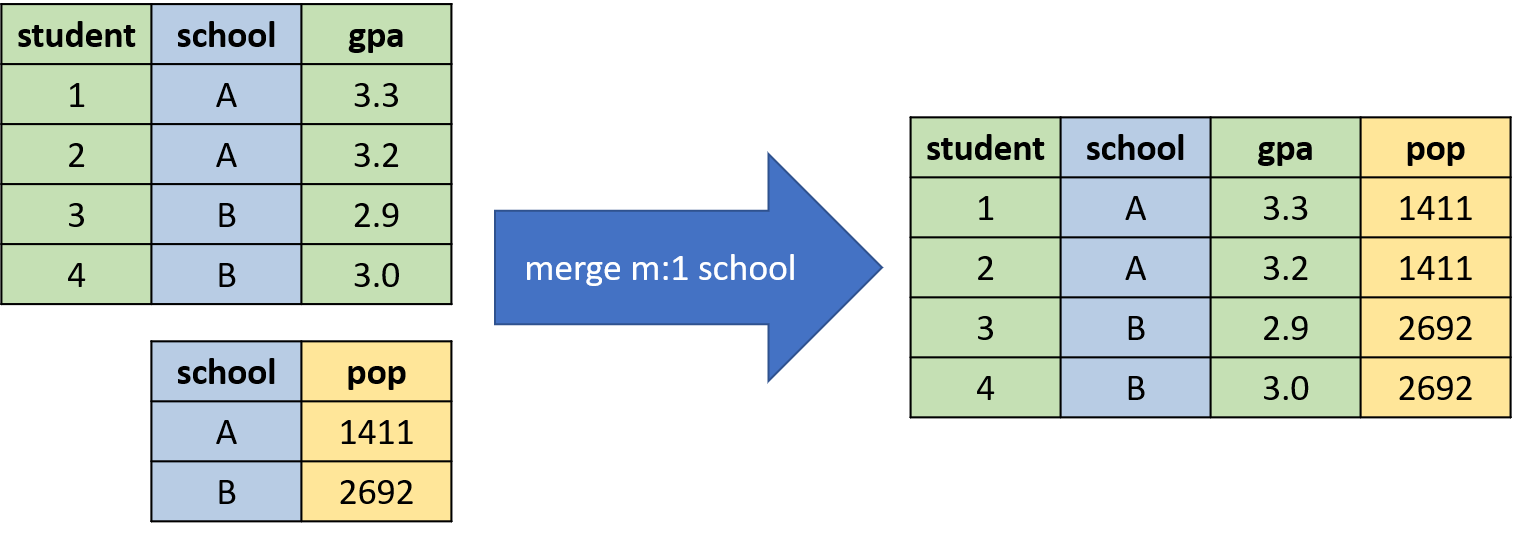
\includegraphics[width=\textwidth]{images/merge_many.png}
\end{center}
\end{frame}


\begin{frame}
\frametitle{Merge 1:m when one table has a coarser unit of analysis}
Depending upon which dataset is used as \textit{master} and which one as \textit{using}, we use \texttt{merge m:1} or \texttt{merge 1:m}
\begin{center}
	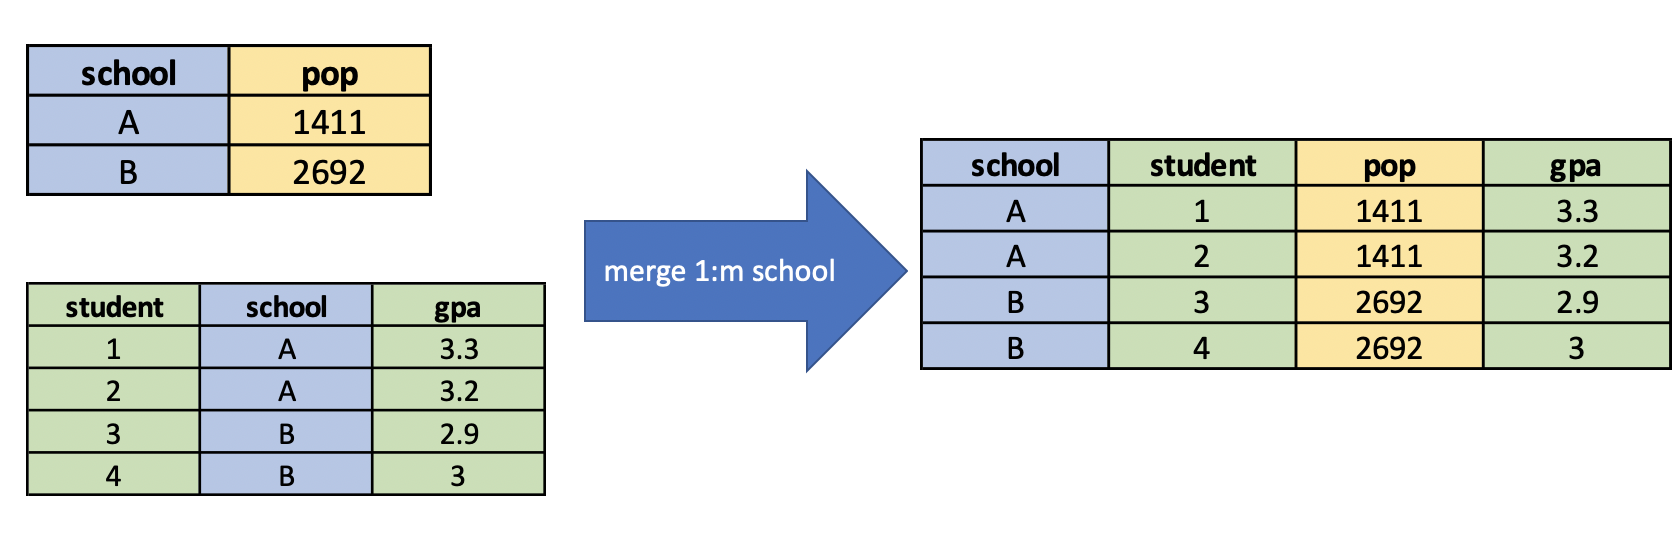
\includegraphics[width=\textwidth]{images/merge}
\end{center}
\pause 
Use \texttt{merge 1:m} when \textit{master} dataset has coarser unit of analysis than \textit{using} data\\
Use \texttt{merge m:1} when \textit{master} dataset has finer unit of analysis than \textit{using} data.
\end{frame}


\begin{frame}
\frametitle{Class exercise: \textit{merge m:1 and 1:m}}
\begin{itemize}
\item Open \texttt{class9.do} 
\item Open \texttt{class9.dta} dataset \\
\bigskip
We'll merge the \texttt{class9.dta} with the \texttt{avg\_annual\_income.dta} in two ways. \\
Verify that \textbf{year-id} is the unique identifier for the first dataset and \textbf{year} for the second one \\
\bigskip
\item \texttt{merge m:1 school}
\item \texttt{merge 1:m school}
\item save as \texttt{class9\_final.dta} file
\end{itemize}
\end{frame}


\begin{frame}
\frametitle{Generating identifiers}
\begin{itemize}
\item[1. ] Create a variable that reflects the unique identifier for \texttt{class9\_final} dataset
%\item[    ] Multiple ways to do this:
\item[1a. ] \texttt{gen unique\_id1= \_n}
\item[1b. ] \texttt{tostring year, gen(yr\_str)}
\item[     ] \texttt{tostring id gen(id\_str)}
\item[     ] \texttt{gen unique\_id2= yr\_str + " " + id\_str}
%\item[1c. ] \texttt{gen unique\_id3= year*10,000,000 + id}
\end{itemize}
\end{frame}


\begin{frame}
\frametitle{Generating identifiers (cont'd)}
\begin{itemize}
\item[2. ] Creating a unique identifier \textbf{for} a group, e.g, year-race
%\item[   ] Multiple ways to do this:
\item[2a.] \texttt{egen id1= group(year white)}
\item[2b.] \texttt{gen id2= year*100 + white}
\bigskip \pause
\item[3. ] Creating a unique identifier \textbf{within} a group, e.g, year
\item[3a.] \texttt{bysort year: gen within\_id= \_n}
\end{itemize}
\end{frame}



\begin{frame}
\frametitle{Here are the commands/operators we covered today:}
\begin{columns}
	\begin{column}{0.5\textwidth}
		\begin{itemize}
			\item \texttt{append}
			\item \texttt{merge 1:1; merge m:1}
			\item \texttt{\_n}
			\item \texttt{bysort}
			\item \texttt{egen}
			\item \texttt{tostring}
			\item \texttt{group}
		\end{itemize}
	\end{column}
	\begin{column}{0.5\textwidth}
	\end{column}
\end{columns}
\end{frame}

\end{document}